\chapter{The Challenge to Succeed (Part 1)}

These notes follow a Jim Rohn seminar talk, preserved here inside the reordered \emph{How You Got Successful?} sequence curated by LazyingArt LLC rather than inside a clean institutional course. The lecture is practical, but it is not loose. It unfolds by a distinct sequence of questions. First, what is the real cost of being present this evening? Next, if two people work under apparently equal conditions, what explains unequal pay? Then, if the world itself does not agree to improve for us, what variable remains under our control? Finally, how do we organize a life once we accept that difficulty, opportunity, defense, and harvest come in recurring cycles?

\section{Opening Contract: Time, Money, and the Right to Teach}

Rohn does not begin with doctrine. He begins with contract. The audience has paid cash to be in the room, but it has also paid in dinner, transportation, arrangements, and above all in time. That is why the opening relation of the evening is not financial in the ordinary sense. It is evaluative:
\begin{equation}
T > M,
\end{equation}
where \(T\) denotes time and \(M\) money.

The point is simple and severe. One can earn more money, but one cannot recover the evening once it has been spent. An evening is a chunk of life. That is why the seminar must justify not only its ticket price but its time price.

This also explains the room-setting that follows. We are told to get paper, borrow some if necessary, and take notes. The session is declared a work session, not entertainment. Even the lighter material at the beginning serves that end. The line about the mind absorbing only what the seat can endure, the practical notice about a break halfway through, the brief exchange with the teenagers in the audience, and the comic schoolboy story all do the same job: they settle the room without lowering the standard. The audience is being warmed up, but it is being warmed up for work.

Only after that does the lecture turn autobiographical. Rohn presents himself first as a man from Idaho farm country, from a practical family, from an ordinary economic world where money, land, and initiative are visible facts. His parents are still busy, still healthy, still making projects for themselves. He even pauses over a concrete example of their practical timing, buying gold at \(125\) and cashing out at \(680\). But the point of this opening is not inherited wisdom. It is contrast.

By age twenty-five he has already promised more than he can deliver. He has married, spoken in large ambitions, and discovered that the dream has outrun the paycheck. The figure he names, \(57\) dollars on Friday, matters because it gives the disappointment a measure. The repeated phrase ``someday honey'' becomes the lecture's first real warning. Someday better furniture. Someday a car. Someday the promised future. The whole seminar will be an argument against that indefinite postponement.

At that stage he does not yet know what to do. Going back to school is considered and then left hanging. The decisive event is Earl Shoaff. Shoaff enters not simply as an employer but as a man who appears wealthy, happy, and worth listening to. Rohn says explicitly that the best thing Shoaff gave him was not the job itself, but the benefit of a philosophy. That claim is the foundation of the whole chapter. The speaker is not presenting abstract principles from nowhere. He is passing on something first received, then tested, then embodied.

\section{From Shoaff to the Seminar Table of Contents}

Once Shoaff enters the story, the seminar acquires a second theme: disciplined notes as the medium of self-change. Rohn says that Shoaff taught him to jot things down, not to use the mind as a filing cabinet, and to rely on repetition. Good ideas, repeated often enough, take root; later they show up not only in memory but in the bank account, the personality, the language, the dress, and the style of life. We are therefore meant to hear the opening instruction to take notes not as clerical advice but as part of the lecture's own causal model.

Years later, going through those journals in Beverly Hills, Rohn decides to share the material publicly. The first seminar is, by his own account, bad. That matters. The public authority of the lecture is earned by repetition, not assumed at the outset. Little by little the speaking grows into a major enterprise, and the private notes become public material.

Only then does he stop and give the audience the formal table of contents. The board is being used not to derive anything, but to create orientation. We are now told where the lecture will travel.

\begin{figure}[t]
\centering

\includegraphics[width=0.82\linewidth]{lecture_18_figure_03.png}
\caption{Chalkboard outline of the seminar's major subjects. The upper line is partly hidden by the speaker, but the spoken list immediately confirms the intended sequence.}
\end{figure}

The spoken outline gives five subjects in order:
\begin{itemize}
\item Personal Development
\item Basic Laws
\item Goals
\item Diseases of Attitude
\item The Day That Turns Your Life Around
\end{itemize}

The screenshot preserves the vertical layout of the board, which matters because the seminar is consciously presenting itself as a structured evening rather than a stream of remarks. A cleaned reconstruction is useful, but it should remain narrow and list-like.

\begin{figure}[t]
\centering
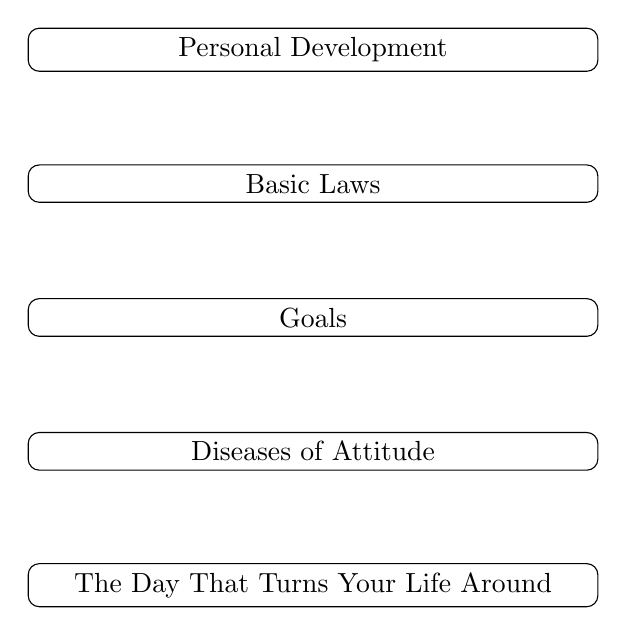
\begin{tikzpicture}
\node[draw, rounded corners, align=center, text width=7cm] at (0,0) {Personal Development};
\node[draw, rounded corners, align=center, text width=7cm] at (0,-1.7) {Basic Laws};
\node[draw, rounded corners, align=center, text width=7cm] at (0,-3.4) {Goals};
\node[draw, rounded corners, align=center, text width=7cm] at (0,-5.1) {Diseases of Attitude};
\node[draw, rounded corners, align=center, text width=7cm] at (0,-6.8) {The Day That Turns Your Life Around};
\end{tikzpicture}
\caption{Transcript-confirmed reconstruction of the board outline.}
\end{figure}

\subsection{Question \& Answer}

\paragraph{Question.} Why does the board begin with personal development rather than with goals or techniques?

\paragraph{Answer.} Because the lecture wants the order to be causal. The person comes before the methods. Rohn says this plainly: if we do not start there, nothing much is going to happen. Goals, laws, attitude, and life-changing days all depend on the quality of the one who acts.

\section{Personal Development as the Upstream Variable}

The first doctrinal move is then made with unusual directness:
\begin{equation}
\text{You can have more than you've got because you can become more than you are.}
\end{equation}
Its companion statement comes immediately:
\begin{equation}
\text{Unless you change how you are, you will always have what you've got.}
\end{equation}

These are not merely motivational slogans. The lecture immediately turns them into a practical law:
\begin{equation}
\text{Income does not far exceed personal development.}
\end{equation}
Sometimes, he admits, income takes a lucky jump. But unless the person grows out to meet that level, it typically falls back. The million-dollar example makes the point concrete: if someone hands us a million dollars, we had better become a millionaire quickly, otherwise the money will disappear. We are not being given a technical market law. We are being shown the lecture's preferred direction of explanation. Stable results require growth in the person who receives them.

A second law follows:
\begin{equation}
\text{Success is something you attract, not something you pursue.}
\end{equation}
Success, in his image, is looking for a good place to stay. That is why the lecture refuses to treat personal development as atmosphere. It is the condition that allows success to remain.

We can now see why the ordinary employment question is rewritten. The major question on the job is not ``What am I getting?'' but ``What am I becoming?'' The point is repeated because it is the hinge between economics and character. The lecture is not anti-income. It is anti-superficial diagnosis. It asks us to inspect the person before the pay.

That is also why happiness is relocated. True happiness, he says, is not contained in what we get. It is contained in what we become. The lecture therefore keeps pressing on the same upstream variable until we see that it is meant to govern income, stability, and even the meaning of work itself.

\paragraph{Mechanism.} In these notes, we may treat personal development as the lecture's hidden variable: the practical condition that constrains retained success, durable performance, and the capacity to use later material about goals and attitude.

\section{Theme of the Seminar and the Compensation Puzzle}

Only after the table of contents and the first doctrine does the lecture pause for its clearest visible maxim. Rohn writes the theme of the seminar on the board and asks the audience not merely to hear it but to keep it in sight during the day.

\begin{figure}[t]
\centering

\includegraphics[width=0.82\linewidth]{lecture_18_figure_04.png}
\caption{The seminar theme written on the board.}
\end{figure}

In cleaned form the line reads:
\begin{equation}
\text{The major key to your better future is you.}
\end{equation}
He asks the audience to underline \emph{major} and \emph{you}. That emphasis matters. Circumstances are not being denied, but the largest controllable term is being identified.

The lecture now turns at once to its most economical puzzle. Why should two people, under apparently equal outward conditions, produce unequal economic results? The matched conditions are deliberately piled up: same company, same products, same services, same traffic, same problems, same community, perhaps even the same age and the same schooling. Yet the monthly outcome differs:
\begin{align}
Y_1 &= 1000 \text{ per month},\\
Y_2 &= 2000 \text{ per month}.
\end{align}
The important question is not what the arithmetic difference is. The important question is what explains it.

At first Rohn allows a false candidate to appear. Perhaps the difference comes from time. Perhaps one person simply has more of it. But that explanation is then rejected, and rejected with humor. There is no stash of extra time hidden anywhere. When the day ends, it ends. In the lecture's compressed notation:
\begin{equation}
T_1 = T_2.
\end{equation}

\subsection{Question \& Answer}

\paragraph{Question.} If time is fixed, what explains the difference in results?

\paragraph{Answer.} The lecture's answer is that time cannot be the missing term. Once the interval and the outward working conditions are held fixed, we must look for some other explanatory variable. The key word introduced at exactly this point is \emph{value}.

\section{Value, Performance, and the Change Principle}

The word ``value'' is the pivot of the chapter. Rohn gives it first as a note-taking phrase:
\begin{equation}
\text{Value makes the difference in results.}
\end{equation}
He then sharpens it into what he calls the first lesson of economics:
\begin{equation}
\text{We primarily get paid for value.}
\end{equation}
and restates the same point in a still tighter way:
\begin{equation}
\text{You get paid for the value, not the time.}
\end{equation}

We can write the lecture's worked example in compressed form. If we hold time fixed and compare equal outward conditions, then the pay gap is being traced to a difference in value:
\begin{align}
T_1 &= T_2,\\
Y_1 &= 1000 \text{ per month},\\
Y_2 &= 2000 \text{ per month}.
\end{align}
The lecture's editorial shorthand may then be written as
\begin{equation}
T=\text{const},\qquad V\uparrow \Rightarrow Y\uparrow,
\end{equation}
with the explicit warning that this is our compression of the spoken reasoning, not notation supplied by Rohn himself.

The same compression lets us express the next question he asks. Can one become twice as valuable and make twice as much money in the same time? Three times as valuable and three times as much money in the same time? In note form:
\begin{align}
V_2 = 2V_1 &\Rightarrow Y_2 \approx 2Y_1,\\
V_2 = 3V_1 &\Rightarrow Y_2 \approx 3Y_1.
\end{align}
Again, this is not a full wage theory. It is a disciplined way of retaining the lecture's practical point: the relevant variable is not additional hours, but higher value brought to the marketplace.

\begin{figure}[t]
\centering
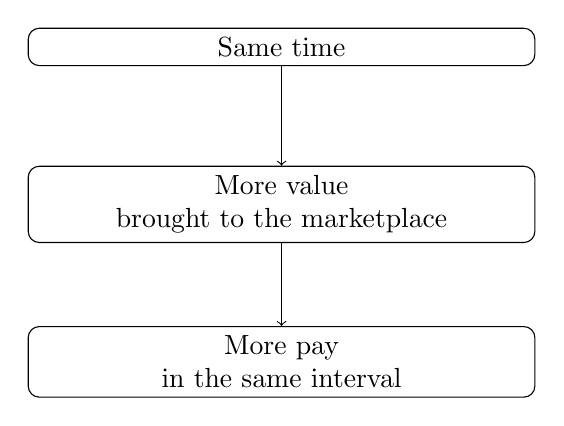
\begin{tikzpicture}
\node[draw, rounded corners, align=center, text width=6.2cm] (t) at (0,0) {Same time};
\node[draw, rounded corners, align=center, text width=6.2cm] (v) at (0,-2.0) {More value\\brought to the marketplace};
\node[draw, rounded corners, align=center, text width=6.2cm] (y) at (0,-4.0) {More pay\\in the same interval};
\draw[->] (t) -- (v);
\draw[->] (v) -- (y);
\end{tikzpicture}
\caption{Pocket-scale schematic of the lecture's compensation argument.}
\end{figure}

Now the lecture widens from economic explanation to ordinary conduct. When asked how to develop an above-average income, Rohn answers: become an above-average person. The examples are intentionally concrete and humble: better handshake, better smile, more excitement, more interest in other people, more intensity to win. The point is that ``value'' is not left abstract. It has behavioral content.

This is also the point at which he clears away three false directions for improvement. One can try to work on the boss. One can try to strike for little increments. One can try to use tricks in sales. All three are rejected as unstable or degrading. The real line is different:
\begin{equation}
\text{It is performance that counts.}
\end{equation}
and then, in the sentence that gives this section its depth,
\begin{equation}
\text{Performance comes from inside, not outside.}
\end{equation}

That is why Shoaff's most famous instruction enters precisely here:
\begin{equation}
\text{Work harder on yourself than you do on your job.}
\end{equation}
Rohn says that when he first heard this he suddenly understood why he was broke. He had been a hard worker on the job. The problem was not effort in general. The problem was effort directed at the wrong object.

\subsection{Question \& Answer}

\paragraph{Question.} If the world itself does not change for us, how can our life change?

\paragraph{Answer.} The lecture's answer is severe and memorable:
\begin{equation}
\text{For things to change for you, you have to change.}
\end{equation}
This is not said once and left alone. It is supported by examples of recurrence: the tide comes in and goes out, day turns to night, winter follows fall, and the next decade is largely ``about like it's always been.'' The point is not pessimism. It is the relocation of the variable. The lecture then compresses the same answer still further:
\begin{equation}
\text{The only way it gets better for you is when you get better.}
\end{equation}

\section{The Seasonal Model and the Four Major Lessons}

Once the change principle has been stated, the lecture reorganizes itself by a larger structure. Before giving the four lessons, Rohn gives two phrases:
\begin{equation}
\text{Life and business are like the changing seasons.}
\end{equation}
\begin{equation}
\text{You cannot change the seasons, but you can change yourself.}
\end{equation}
These two lines gather the previous argument into one model. The first names the recurrent external order. The second isolates the internal variable that remains open to us.

\begin{figure}[t]
\centering
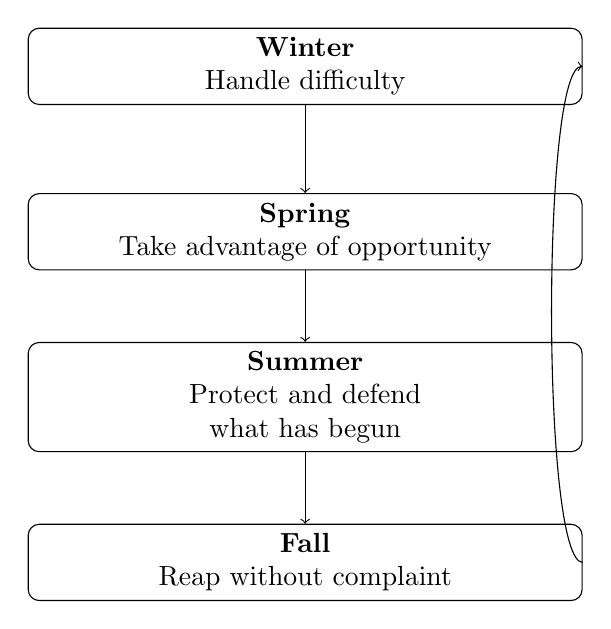
\begin{tikzpicture}
\node[draw, rounded corners, align=center, text width=6.8cm] (w) at (0,0) {\textbf{Winter}\\Handle difficulty};
\node[draw, rounded corners, align=center, text width=6.8cm] (sp) at (0,-2.1) {\textbf{Spring}\\Take advantage of opportunity};
\node[draw, rounded corners, align=center, text width=6.8cm] (su) at (0,-4.2) {\textbf{Summer}\\Protect and defend\\what has begun};
\node[draw, rounded corners, align=center, text width=6.8cm] (f) at (0,-6.3) {\textbf{Fall}\\Reap without complaint};
\draw[->] (w) -- (sp);
\draw[->] (sp) -- (su);
\draw[->] (su) -- (f);
\draw[->] (f.east) .. controls (3.0,-6.3) and (3.0,0.0) .. (w.east);
\end{tikzpicture}
\caption{Compact reconstruction of the lecture's seasonal cycle.}
\end{figure}

In compressed form we may write
\begin{equation}
\text{Winter} \to \text{Spring} \to \text{Summer} \to \text{Fall} \to \text{Winter}.
\end{equation}
This is not a formal state model. It is the lecture's structural picture of recurring life conditions.

The four lessons then unfold in order.

\begin{enumerate}
\item \textbf{Learn how to handle the winters.} Difficulty is inevitable. Nights follow days, recessions follow progressions, and winter follows fall. We cannot tear January off the calendar and thereby remove it. So the instruction is not to wish winter away, but to grow strong enough to meet it. This is the place where Shoaff's maxim appears:
\begin{equation}
\text{Do not wish it were easier; wish you were better.}
\end{equation}
The lecture immediately extends it: do not wish for fewer problems, wish for more skills; do not wish for less challenge, wish for more wisdom.

\item \textbf{Learn how to take advantage of the spring.} Spring is opportunity, and opportunity follows difficulty. But spring does not do the work for us. One must take advantage. One must plant. ``Planting in the spring or begging in the fall'' is the lecture's deliberately sharp contrast. Opportunity is not enough; it has to be used, and used promptly, because there are only so many springs.

\item \textbf{Learn how to protect your crops all summer.} Here the lecture introduces two laws of defense:
\begin{equation}
\text{All good will be attacked.}
\end{equation}
\begin{equation}
\text{All values must be defended.}
\end{equation}
Every garden is invaded. Every value requires tending. Summer is therefore the season of vigilance and maintenance.

\item \textbf{Learn how to reap in the fall without complaint.} Harvest is the season of responsibility. If we do well, there is no need to apologize. If we do poorly, there is no permission to complain. In either case, maturity lies in accepting responsibility for the harvest.
\end{enumerate}

\subsection{Question \& Answer}

\paragraph{Question.} How do we handle winter, and what do we do when spring comes?

\paragraph{Answer.} We do not handle winter by denying it. We handle it by becoming stronger, wiser, and better. Then, when spring comes, we do not merely admire it. We plant in it, move quickly, and use it before it passes. The lecture's point is that the seasons themselves are fixed; the quality of our participation in them is not.

\section{Not What Happens, but What We Do}

After the four lessons, the lecture does not relax. It turns back, sharply, to the human habit of explanation. Rohn says he once carried a long list of reasons he was not doing well: government, taxes, prices, weather, traffic, the car, the company, company policy, the training program, relatives, neighbors, the economy, the community. The list is humorous, but not trivial. It is the ordinary logic of blame written out in public.

Shoaff's interruption is brutal and exact: the big problem with the list is that Rohn is not on it. The list is torn up, and a fresh page is imagined with one word on it: \emph{Me}. This is the moment at which the lecture states the next major law:
\begin{equation}
\text{It is not what happens; it is what you do.}
\end{equation}
The supporting gloss is equally important:
\begin{equation}
\text{What happens is about the same; what people do is what is different.}
\end{equation}

The garbled line in the transcript around this point is clarified by the repeated surrounding statements. The lecture's meaning is steady: events do not by themselves determine the quality or quantity of a life because the same events can meet different responses.

This is why Murphy's laws can be admitted without surrender. Anything can happen. Everything can go wrong. One can lose a fortune, watch things collapse, see it all go. But these are still happenings. They do not yet settle the question of outcome. Likewise disappointment is not a special gift reserved for the poor. Everybody gets a share. The difference remains response.

The rainstorm example gives the lecture's cleanest local demonstration:
\begin{enumerate}
\item One man sees the storm and stays home. For him, the storm is a reason not to sell.
\item Another man sees the same storm and goes out. For him, the storm is a chance to find people at home and competitors absent.
\end{enumerate}
The weather is common. The reading of the weather is not. And once the reading changes, the action changes.

This section also recovers the lecture's moral sharpness. Once happenings are treated as shared, personal disappointment can no longer function as a sovereign excuse. The law remains:
\begin{equation}
\text{It is not what happens; it is what you do about it.}
\end{equation}

\subsection{Question \& Answer}

\paragraph{Question.} What can we do starting tomorrow that will make a difference?

\paragraph{Answer.} Here the lecture deliberately leaves us under pressure rather than offering a neat program. If we do nothing tomorrow that changes direction, then the next five years will tend to look like the last five. That is the negative answer. The positive answer is smaller and more demanding: change something real. Change a habit, a discipline, a use of time, a standard of self-work, an act of initiative. The lecture insists that any day we wish, we can change our whole life; but it also insists that this does not happen by mood. It happens when tomorrow ceases to be a repetition of today.

\section{Summary}

The lecture unfolds by a strict internal sequence. An evening is more valuable than the money spent to attend it, so the session must become work. Because time is fixed, the compensation puzzle directs us to value rather than duration. Because value depends on the person who acts, we are told to work harder on ourselves than on the job. Because the world itself is not obligated to improve for us, change must begin in us. Because life and business move in seasons, wisdom means learning how to handle winter, use spring, defend summer, and reap fall responsibly. And because happenings are widely shared, the decisive term is finally neither circumstance nor complaint, but response.

Part 1 therefore closes as the seminar closes: not with a completed system, but with a practical challenge. Tomorrow is the first place where the lecture can be either confirmed or ignored.